\section*{HOW TO (Remove this whole section !!!)}
\label{sec:usage}

The purpose of this document structure is to ensure compatibility between all documents across all groups. Therefore, you are limited to this template. Our goal is to create a single document across all \textit{p3 Project Reports}.

\medskip
This template is used for the student reports of the \coursename\ course. Remove this section by editing the \texttt{reportContent.tex} file \textbf{after} you have understood how to use this template.

\medskip
\textbf{Note:} If you use this file as your template, make sure to replace \verb|\section*{}| and \verb|\subsection*{}| with \verb|\section{}| and \verb|\subsection{}| respectively. We did purposely use the non-numbered sections in this guide, however in your report the numbered sections are better suited.

\subsection*{Folder Structure}
\begin{lstlisting}[escapechar=!,basicstyle=\footnotesize]
proceedings /
  |- reportContent /  <-- YOUR working folder
      |- images /     <-- Images are stored here
      |- sections /   <-- Place sections / tex-files here
          |- introduction.tex
          |- report.bib
          |- lessons-learned.tex
          '- section2.tex
      '- reportContent.tex  <-- Change section imports here
  |- !\rootDocument!  <-- DO NOT alter this file
  |- _HOWTO_.tex    <-- *this* How To section
  |- llncs.cls                            <-- NOR that
  |- proceedings.py                       <-- NOR that
  |- splncs03.bst                         <-- NOR that
  '- UniBas_Logo_EN_Schwarz_RGB_65.pdf    <-- NOR that
\end{lstlisting}


\newpage
\subsection*{Setup}
\begin{samepage}
    Your report is compiled using the \texttt{\rootDocument} file. Therefore, we suggest that you set the file \texttt{\rootDocument} as the Master-/Root-Document that you can conveniently work on your report.
    Please be aware that you have to compile the \texttt{\rootDocument} file in the following order:
    
    \begin{enumerate}
        \item \verb|pdflatex| \rootDocument
        \item \verb|biber| \rootName
        \item \verb|pdflatex| \rootDocument
        \item \verb|pdflatex| \rootDocument
    \end{enumerate}
\end{samepage}


For your convenience, you can compile this document by using the \texttt{proceedings.py} utility:

\begin{center}
    \verb|$> python proceedings.py -p|
\end{center}

And subsequently (especially before your submission) clean the auxiliary \LaTeX\ files:

\begin{center}
    \verb|$> python proceedings.py -z|
\end{center}

Additionally, this template is compatible with Overleaf. You can simply upload the zip as a new project.



\subsection*{Images}
Images placed in the \texttt{images} sub-folder can be used directly in the \texttt{\textbackslash includegraphics} command -- see also \Cref{fig:rosette}. Also, sub-figures are possible: \Cref{fig:fly,fig:flies}.

Please \textsc{do~not} store your images elsewhere! 

Please use your group number (e.g., \textit{1}) in every image file name (e.g., \textit{g1-rosette.pdf} instead of \textit{rosette.pdf})!

\textbf{It is mandatory, that you do \emph{only} specify the filename, as the path is set automatically.} Hence, for \Cref{fig:rosette}, the command to include the image is \verb|
\includegraphics{g1-rosette}|

\begin{figure}[!ht]
\centering

\includegraphics[width=0.45\textwidth]{g1-rosette}
\caption{Example figure stored in the \texttt{images} sub-folder and displayed with \texttt{\textbackslash includegraphics[width=0.45\textbackslash textwidth]\{g1-rosette\}}}
\label{fig:rosette}
\end{figure}

%% [H] overwrites float and force image to be here
\begin{figure}[H]
%\begin{figure}[tb]
\centering
    %\subfloat[CAPTION]{BILDERCODE}\qquad
    \subfloat[A fly\label{fig:fly}]{
\includegraphics[width=0.4\textwidth]{g1-fly}}\qquad
    \subfloat[Flies\label{fig:flies}]{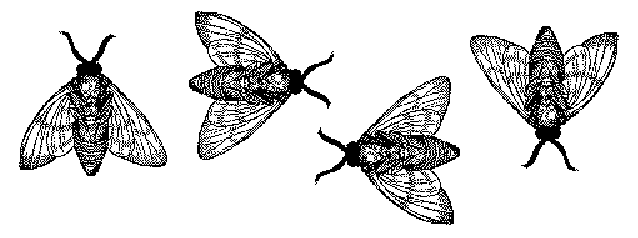
\includegraphics[width=0.45\textwidth]{g1-flies}}
\caption{Example figure stored in the \texttt{images} sub-folder}
\label{fig:example subfigure}
\end{figure}


\subsection*{Code}
To illustrate code use the \texttt{lstlisting} environment:

\begin{lstlisting}[language={Java}, label={lst:javaexample}, captionpos=b, caption={Example for Java}]
public void foo( final int bar ) {
  System.out.println( bar );
}
\end{lstlisting}


\begin{lstlisting}[language={Python}, label={lst:pythonexample}, captionpos=b, caption={Example for Python}]
x = 1
if x == 1:
   print("x is 1.")
\end{lstlisting}


\begin{lstlisting}[language={SQL}, label={lst:sqlexample}, captionpos=b, caption={Example for SQL}]
SELECT * FROM users;
\end{lstlisting}


\subsection*{External PDF}
One can also easily import a PDF document using\smallskip

\verb|\includepdf[pages=1,pagecommand={\pagestyle{headings}}]{filename}| \smallskip

to include the \verb|filename.pdf| document.
It is important to use the pagestyle \emph{fancy}, so that the header is also on the included page. Furthermore, please ensure that your PDF version (or image) of the ER diagram is \textbf{readable}.


\subsection*{Labels and References}
The proceedings template includes the package \textit{cleveref}, which enables pretty references. One such reference is the following one: \Cref{fig:example subfigure}, which was produced using the command \verb|\Cref{fig:example subfigure}|.
To use the full potential of such clever referencing, one have to set up labels, such as in the example before. The label command was \verb|\label{fig:example_subfigure}| (as seen in the source code in line 69).
Be aware that you have to prefix every single label you use with your group name, i.e. \verb|g1| to not clash with other group's labels.

\subsection*{Bibliography}
We use the \verb|biblatex| package with biber\footnote{\url{http://biblatex-biber.sourceforge.net/}} as backend, which most distributions already include.
Your references are stored in the \texttt{report.bib} file and used with the \texttt{\textbackslash cite} command. 
For example: \cite{kopka1995guide}. 
If the previous example shows \verb|kopka1995guide| - you need to re-run the compilation in the following order: pdflatex, biber, pdflatex, pdflatex.
In case you need some help with references in latex, there is an excellent cheatsheet\footnote{\url{http://tug.ctan.org/info/biblatex-cheatsheet/biblatex-cheatsheet.pdf}}.

\newpage
\subsection*{Tikz Drawing}

Yon can also integrate ER diagrams using \LaTeX and Ti\textit{k}Z (instead of importing the PDF).

\label{gX-sec:tutorial}
\begin{center}
	\begin{tikzpicture}[
		every entity/.style={draw=green, fill=green!10, text=black},
		every attribute/.style={draw=blue, fill=blue!10, text=black},
		every relationship/.style={draw=yellow, fill=yellow!10, text=black},
		node distance=8em
		]
		%% Entity One
		\node[entity](e1){EntityOne};
		\node[attribute](e1id)[above left of=e1]{\underline{primary\_key}} edge (e1);
		\node[attribute](att1)[above of=e1]{attribute1} edge (e1);
		\node[attribute](att2)[above right of=e1]{attribute2} edge (e1);
		
		%% Relation, including cardinality
		\node[relationship](rel)[right of=e1]{relates\_to} edge node [auto,swap]{(0,*)}(e1);
		
		%% Entity Two, includinig cardinality
		\node[entity](e2)[right of=rel]{EntityTwo} edge node [auto,swap] {(0,1)}(rel);
		\node[attribute](e2id)[above of=e2]{\underline{e2\_id}} edge (e2);
		\node[attribute](e2attr)[above right of=e2]{attribute1} edge (e2);
		
		%% Entity Three, with an IS-A relation to Entity Two (i.e. inheritance)
		\node[entity](e3)[below of=e2]{EntityThree};
		\node[attribute](e3attr)[below left of=e3]{attribute2} edge (e3);
		% For Specialization: e3 is a specialization of e2 (i.e. a child of)
		\draw[double distance=.05cm,-Triangle] (e3) -- (e2); % You might want to adjust the double distance value
		
		%% WEAK Relation, with WEAK Entity
		\node[relationship, double distance=.02cm](rel2)[below of=e1]{consists\_of} edge node[auto,swap]{(0,1)}(e1);
		\node[entity, double distance=.02cm](e4)[below of=rel2]{EntityFour} edge node[auto, swap] {(1,1)}(rel2);
		\node[attribute](e4id)[above left of=e4]{\underline{id}} edge (e4);
		\node[attribute](e4attr2)[left of=e4]{attribute} edge (e4);
	\end{tikzpicture}
\end{center}


\newpage
\subsection*{Allowlist}
Below you will find a \emph{Allowlist} of all available latex packages. These packages should be sufficient for the creation of your document. If other packages are necessary, this must be clarified with the tutor in advance.

\begin{lstlisting}[language={[LaTeX]TeX}, label=lst:Internationalization, basicstyle=\footnotesize]
%% Internationalization Latex Settings
\usepackage[ngerman,english]{babel}
\selectlanguage{english}

% Choose the encoding of the input text. 
\usepackage[utf8]{inputenc}
% To choose the font encoding of the output text. 
\usepackage[T1]{fontenc}
\end{lstlisting}

\begin{lstlisting}[language={[LaTeX]TeX}, label=lst:Bibliography, basicstyle=\footnotesize]
%% Packages for Bibliography
\usepackage{csquotes}
% Recommended for biblatex
\usepackage{xpatch} 
% pdflatex -> biber -> pdflatex (2x)
\usepackage[backend=biber,style=numeric,language=english]{biblatex}
\end{lstlisting}

\begin{lstlisting}[language={[LaTeX]TeX}, label=lst:Lists, basicstyle=\footnotesize]
%% Lists
\usepackage{mdwlist}
\usepackage{paralist}
\usepackage{enumitem}
\renewcommand\labelitemi{--}
\end{lstlisting}


\begin{lstlisting}[language={[LaTeX]TeX}, label=lst:Float, basicstyle=\footnotesize]
%% Floats
\usepackage{float}
% Adds Float \FloatBarrier beyond which floats may not pass
\usepackage[section]{placeins}
\end{lstlisting}

\begin{lstlisting}[language={[LaTeX]TeX}, label=lst:Images, basicstyle=\footnotesize]
%% Images
% Allows you to insert graphic files within a document. 
\usepackage{graphicx}
\usepackage[justification=centerlast, font=small]{caption}
\usepackage{subcaption}
%\usepackage[caption=false]{subfig}
\end{lstlisting}

\begin{lstlisting}[language={[LaTeX]TeX}, label=lst:Tables, basicstyle=\footnotesize]
%% Tables
\usepackage{array}
\usepackage{tabularx}
\usepackage{booktabs}
% For Tables longer than one Page
\usepackage{longtable} 
\usepackage{multirow}
\usepackage{makecell, boldline}
\end{lstlisting}

\begin{lstlisting}[language={[LaTeX]TeX}, label=lst:Math, basicstyle=\footnotesize]
%% Math
\usepackage{mathtools}
\usepackage{amsfonts}
%\usepackage{amsthm}% Incompatible with document
\usepackage{amssymb}
\usepackage{xfrac}
\end{lstlisting}


\begin{lstlisting}[language={[LaTeX]TeX}, label=lst:Code, basicstyle=\footnotesize]
%% Code
% For Algorithms
\usepackage{algorithmic}
\usepackage{algorithm}

% Plain code printing
\usepackage{listings} 
\usepackage{verbatim}

\end{lstlisting}

\begin{lstlisting}[language={[LaTeX]TeX}, label=lst:Colors, basicstyle=\footnotesize]
%% For Colors (\textcolor etc.)
\usepackage{color}
\usepackage{xcolor}
\end{lstlisting}


\begin{lstlisting}[language={[LaTeX]TeX}, label=lst:Tikz, basicstyle=\footnotesize]
%% For Tikz
\usepackage{tikz}
% A library providing ER prefabs
\usetikzlibrary{er}
\usetikzlibrary{positioning,arrows.meta}
\end{lstlisting}

\begin{lstlisting}[language={[LaTeX]TeX}, label=lst:References, basicstyle=\footnotesize]
%% References
% For URLs
\usepackage{xurl}
% Refs
\usepackage{appendix}
\usepackage{varioref}
\usepackage[
colorlinks,        % Links without boarder
linkcolor=black,   % Color internal links
filecolor=black,   % Color external links
citecolor=black,   % Cite Color
urlcolor=black	   % URL Color
]{hyperref}
\usepackage{cleveref}
\end{lstlisting}

\begin{lstlisting}[language={[LaTeX]TeX}, label=lst:Import, basicstyle=\footnotesize]
%% Import
% For input external files
\usepackage{import}
% Import of external PDF's
\usepackage{pdfpages}
\end{lstlisting}


\begin{lstlisting}[language={[LaTeX]TeX}, label=lst:Tools, basicstyle=\footnotesize]
%% Further tools and styles
% For dummy text generation
\usepackage{lipsum}
% Support for setting the spacing between lines
\usepackage{setspace}
% For Todo Notes 
\usepackage[colorinlistoftodos]{todonotes}
% For curly underline
\usepackage[normalem]{ulem}
\end{lstlisting}





\pagebreak
